%!TEX root = ../thesis.tex
%*******************************************************************************
%*********************************** Fifth Chapter *****************************
%*******************************************************************************

\chapter{Smoothing}
\ifpdf
    \graphicspath{{Chapter5/Figs/Raster/}{Chapter5/Figs/PDF/}{Chapter5/Figs/}}
\else
    \graphicspath{{Chapter5/Figs/Vector/}{Chapter5/Figs/}}
\fi
Topological objects are inherently geometric in nature, and as a result they can suffer substantially from ambiguities brought about by the discretisation of spacetime. Hence, when considering the behaviour of topological objects on the lattice, it has been proven to be necessary to remove high frequency fluctuations in the gauge fields~\cite{Bonnet:2000dc}. Furthermore, when investigating the long distance behaviour of the lattice it is also beneficial to filter off the short distance fluctuations to better reveal the physics in the region of interest~\cite{Moran:2008ra}. The process of removing these fluctuations is known as smoothing, which in turn falls into two sub-categories: cooling and smearing.\\

The purpose of both these methods is similar, however, the algorithms used to implement them differ greatly. Cooling assesses each link, replacing the existing link with one that locally minimises some choice of action (see e.g. the Wilson action in Eq.~\ref{eq:WilsonAction}). Smearing does not depend on the choice of action, and instead replaces each link with a weighted average of its nearest neighbours. Once every link in the lattice has been updated, the configuration is said to have had one sweep of smoothing applied. The process can then be repeated to an arbitrary number of sweeps.  Due to the differences in the routines, it is important to compare the results from both to observe how they each perform and quantitatively observe how the alter the measured quantities.

\section{Smoothing Methods}
\subsection{Cooling}
\subsection{Over-Improved Smearing}

\section{Results from the Gluon Propagator}\label{sec:CoolingGluProp}
It has previously been shown that smoothing is necessary to obtain agreement between the untouched and vortex only string tension, mass function and instanton content~\cite{Trewartha:2015ida,Trewartha:2015nna,Trewartha:2017ive}. Motivated by these results, we now investigate the effect of both $\mathcal{O}(a^4)$-improved cooling~\cite{BilsonThompson:2003zi} and over-improved stoutlink smearing~\cite{Moran:2008ra}. Following the results of Ref.~\cite{Moran:2008ra}, the over-improved smearing parameters are $\rho=0.06$ and $\epsilon=0.25$ to best preserve the size of instantons on the lattice. To accomplish a similar preservation of topological objects under cooling, we used the three-loop improved algorithm as described in Ref.~\cite{BilsonThompson:2003zi}.\\
%
\begin{figure}[tb]
\centering
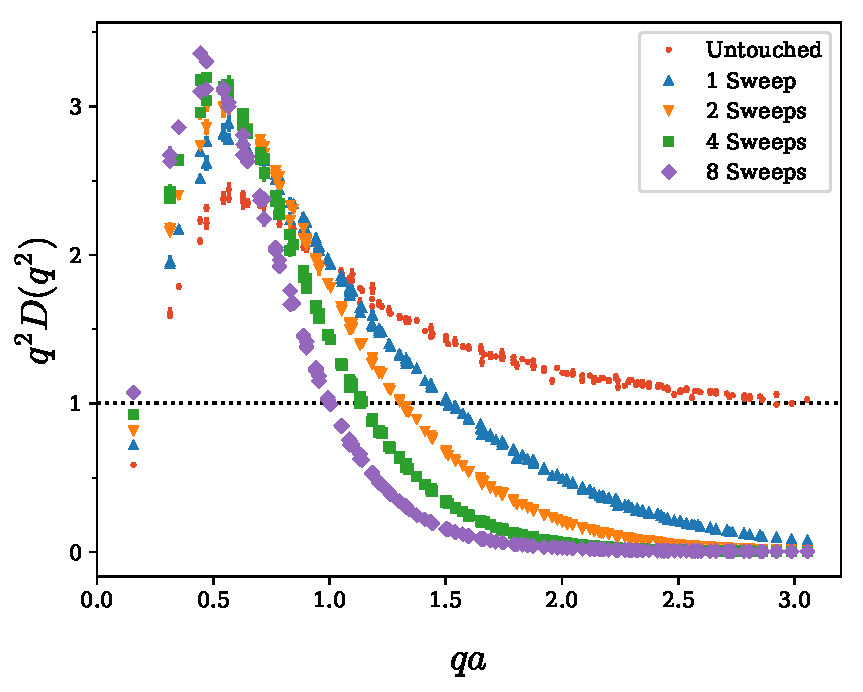
\includegraphics[width=\linewidth]{./ScalarGluComp_q2_1to10sweeps.pdf}
\caption{\label{fig:1to10SweepsCooling}Comparison of the gluon propagator on the untouched configurations after cooling. For clarity we have selected a sample of sweeps between 1 and 8.}
\end{figure}
%

We first plot the untouched propagator after 0, 1, 2, 4 and 8 sweeps of cooling in Fig.~\ref{fig:1to10SweepsCooling}. In gauge fixing, each sweep has been preconditioned by the Landau gauge transformation of the prior sweep in descending order (i.e. the transformation for sweep 10 preconditions sweep 9). This preconditioning is done to ensure that the Landau gauge functional is near the same local minima for each cooling sweep. We observe the expected removal of short distance fluctuations that is typical of smoothing, resulting in a suppressed propagator at large $q$. This is complemented by an amplification in the infra-red region which can be attributed to the increase in low momentum modes arising from the smoothing of the gauge fields.\\
%
\begin{figure}[tb]
\centering
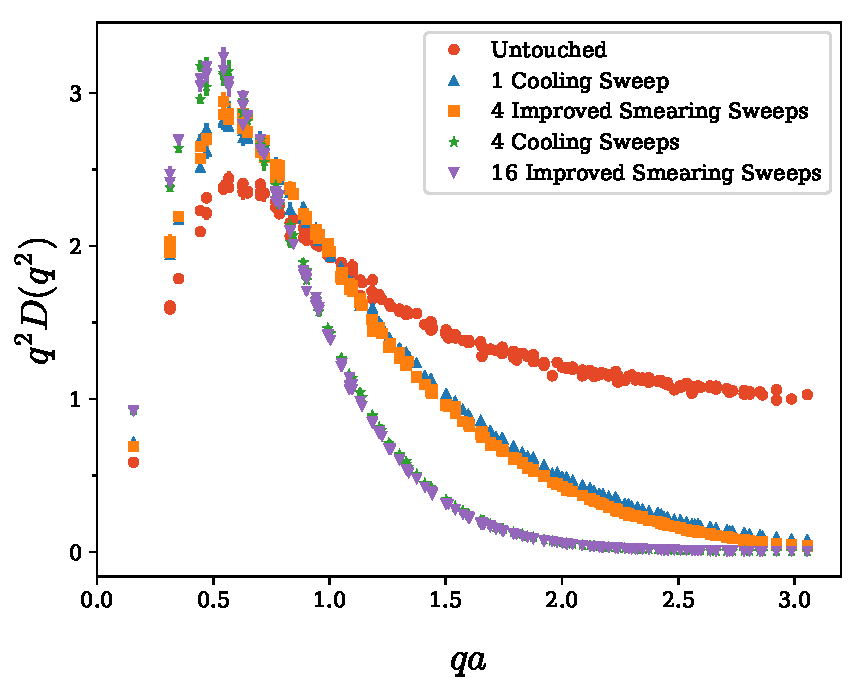
\includegraphics[width=\linewidth]{./ScalarGluComp_q2_SmearCoolComp.pdf}
\caption{\label{fig:SmearCoolComp}The gluon propagator after cooling or improved smearing. We see that the shape of the plot changes minimally between the smoothing routines. However cooling requires fewer sweeps to produce the same effect when compared to smearing.}
\end{figure}
%

To compare the effects of cooling and over-improved smearing, the untouched gluon propagator is plotted in Fig.~\ref{fig:SmearCoolComp} after either over-improved smearing or cooling. By comparing the smeared and cooled propagator we can see that cooling has a more rapid effect, related to the well-known fast removal of action from the lattice. The qualitative shape of the propagator remains the same however, and it can be seen that, for example, 4 smearing sweeps produces a propagator remarkably similar to 1 cooling sweep. More generally, we observe that in regards to the shape of the propagator, $n_{\text{sm}}\approx4\,n_{\text{cool}}$. Following the observation made in Ref.~\cite{Thomas:2014tda} that the number of over-improved stoutlink smearing sweeps is related to the gradient flow time by
%
\begin{equation}
t\approx\rho\,n_{\text{sm}}\, ,
\end{equation}
%
we deduce that the relationship between gradient flow time and cooling is
\begin{equation}
t\approx0.24\,n_{\text{cool}}\,.
\end{equation}\\

It is well understood that smoothing alters the vortex background, and based on previous work~\cite{Cais:2008za,Trewartha:2015ida,DelDebbio:1998luz} we anticipate that the vortices identified on smoothed configurations would differ to those identified on the unsmoothed configurations. We therefore perform vortex identification only on the original configurations, with smoothing then being performed independently on the untouched, vortex-only and vortex-removed configurations. We choose to use cooling as the smoothing algorithm for the results presented in this paper, however it is worth noting that similar results can be obtained with the use of over-improved smearing. 

